\documentclass{article}

% if you need to pass options to natbib, use, e.g.:
%     \PassOptionsToPackage{numbers, compress}{natbib}
% before loading neurips_2025

% The authors should use one of these tracks.
% Before accepting by the NeurIPS conference, select one of the options below.
% 0. "default" for submission
\usepackage[preprint]{neurips_2025}
% the "default" option is equal to the "main" option, which is used for the Main Track with double-blind reviewing.
% 1. "main" option is used for the Main Track
%  \usepackage[main]{neurips_2025}
% 2. "position" option is used for the Position Paper Track
%  \usepackage[position]{neurips_2025}
% 3. "dandb" option is used for the Datasets & Benchmarks Track
 % \usepackage[dandb]{neurips_2025}
% 4. "creativeai" option is used for the Creative AI Track
%  \usepackage[creativeai]{neurips_2025}
% 5. "sglblindworkshop" option is used for the Workshop with single-blind reviewing
 % \usepackage[sglblindworkshop]{neurips_2025}
% 6. "dblblindworkshop" option is used for the Workshop with double-blind reviewing
%  \usepackage[dblblindworkshop]{neurips_2025}

% After being accepted, the authors should add "final" behind the track to compile a camera-ready version.
% 1. Main Track
 % \usepackage[main, final]{neurips_2025}
% 2. Position Paper Track
%  \usepackage[position, final]{neurips_2025}
% 3. Datasets & Benchmarks Track
 % \usepackage[dandb, final]{neurips_2025}
% 4. Creative AI Track
%  \usepackage[creativeai, final]{neurips_2025}
% 5. Workshop with single-blind reviewing
%  \usepackage[sglblindworkshop, final]{neurips_2025}
% 6. Workshop with double-blind reviewing
%  \usepackage[dblblindworkshop, final]{neurips_2025}
% Note. For the workshop paper template, both \title{} and \workshoptitle{} are required, with the former indicating the paper title shown in the title and the latter indicating the workshop title displayed in the footnote.
% For workshops (5., 6.), the authors should add the name of the workshop, "\workshoptitle" command is used to set the workshop title.
% \workshoptitle{WORKSHOP TITLE}

% "preprint" option is used for arXiv or other preprint submissions
 % \usepackage[preprint]{neurips_2025}

% to avoid loading the natbib package, add option nonatbib:
%    \usepackage[nonatbib]{neurips_2025}

\usepackage{hyperref}       % hyperlinks
\usepackage{url}            % simple URL typesetting
\usepackage{booktabs}       % professional-quality tables

\usepackage{graphicx}
% Layout tweaks for tighter, professional look (after graphicx loaded)
\usepackage[skip=4pt, font=small]{caption}
\usepackage{subcaption}
\captionsetup[subfigure]{skip=2pt, font=footnotesize}
\setlength{\textfloatsep}{6pt plus 2pt minus 2pt}
\setlength{\floatsep}{6pt plus 2pt minus 2pt}
\setlength{\intextsep}{6pt plus 2pt minus 2pt}
\setlength{\abovecaptionskip}{4pt}
\setlength{\belowcaptionskip}{2pt}
\setlength{\parskip}{2pt}

% Tighter section spacing
\usepackage{titlesec}
\titlespacing*{\section}{0pt}{8pt plus 2pt minus 2pt}{4pt plus 1pt minus 1pt}
\titlespacing*{\subsection}{0pt}{6pt plus 2pt minus 2pt}{3pt plus 1pt minus 1pt}

% Image rendering quality (after graphicx)
\graphicspath{{figures/}}
\DeclareGraphicsExtensions{.png,.pdf,.jpg}

\usepackage{amsfonts}       % blackboard math symbols
\usepackage{nicefrac}       % compact symbols for 1/2, etc.
\usepackage{microtype}      % microtypography
\usepackage{xcolor}         % colors

% Note. For the workshop paper template, both \title{} and \workshoptitle{} are required, with the former indicating the paper title shown in the title and the latter indicating the workshop title displayed in the footnote. 
\usepackage{fontspec}
\setmainfont{Times New Roman}
\setsansfont{Arial}
\setmonofont{Courier New}


\usepackage{enumitem}
\usepackage{float}

\title{Datathon 2026 -- Round 1: EDA \& Sales Forecasting for Vietnamese Fashion E-commerce}


% The \author macro works with any number of authors. There are two commands
% used to separate the names and addresses of multiple authors: \And and \AND.
%
% Using \And between authors leaves it to LaTeX to determine where to break the
% lines. Using \AND forces a line break at that point. So, if LaTeX puts 3 of 4
% authors names on the first line, and the last on the second line, try using
% \AND instead of \And before the third author name.


\author{%
  Trần Nam Anh \and Đặng Minh Phát \and Nguyễn Đức Hải \and Ngô Thị Ánh Dương \\
  \textbf{Team: The Richers} \\
  Datathon 2026 -- Round 1 Submission
}
  % examples of more authors
  % \And
  % Coauthor \\
  % Affiliation \\
  % Address \\
  % \texttt{email} \\
  % \AND
  % Coauthor \\
  % Affiliation \\
  % Address \\
  % \texttt{email} \\
  % \And
  % Coauthor \\
  % Affiliation \\
  % Address \\
  % \texttt{email} \\
  % \And
  % Coauthor \\
  % Affiliation \\
  % Address \\
  % \texttt{email} \\


\begin{document}

\maketitle

\begin{abstract}
  Báo cáo EDA và dự báo doanh thu cho e-commerce thời trang Việt Nam giai đoạn 2012--2022, được tổ chức theo \textbf{4 cấp độ Descriptive--Diagnostic--Predictive--Prescriptive}. EDA phát hiện: (i) Streetwear chiếm 75\% portfolio (12.15 tỷ) với concentration risk; (ii) wrong\_size là root cause 35\% returns đồng nhất across category; (iii) COD cancel rate 16\% gấp 2$\times$ online; (iv) tất cả mega sales VN (12.12, Black Friday, 11.11, Tết) đều \textit{giảm} doanh thu 27--49\%; (v) RFM phân 6 segment, Champions 24\% population đóng góp 9.0 tỷ; (vi) Risk Tier classification flag 30 SKUs High Risk (median return 24\%) cần can thiệp Q1 2023. Forecasting đề xuất \textbf{Hybrid Multi-Layer} với cross-table features, macro-event encoding và alpha-shrinkage residual stacking; CV Revenue $R^2$=0.7823, COGS $R^2$=0.7916 trên 2 fold time-series 2021--2022. Top-5 actionable recommendations với expected impact $\sim$1.7--1.8 tỷ tăng doanh thu và $\sim$500 triệu tiết kiệm chi phí/năm.
\end{abstract}

\section{Exploratory Data Analysis}

EDA phân tích 13 bảng (715K orderlines, 647K orders, 87,839 customers, 2,412 SP) qua \textbf{4 cấp độ Descriptive--Diagnostic--Predictive--Prescriptive} trên 3 chủ đề: Product Portfolio, Customer, Promotion/Operations. Dựa trên 5 Data Marts với metric chuẩn hóa (Net Revenue, Gross Margin, Return Rate qty-based).

\subsection{Descriptive: Portfolio \& Customer Snapshot}

\begin{figure}[H]
    \centering
    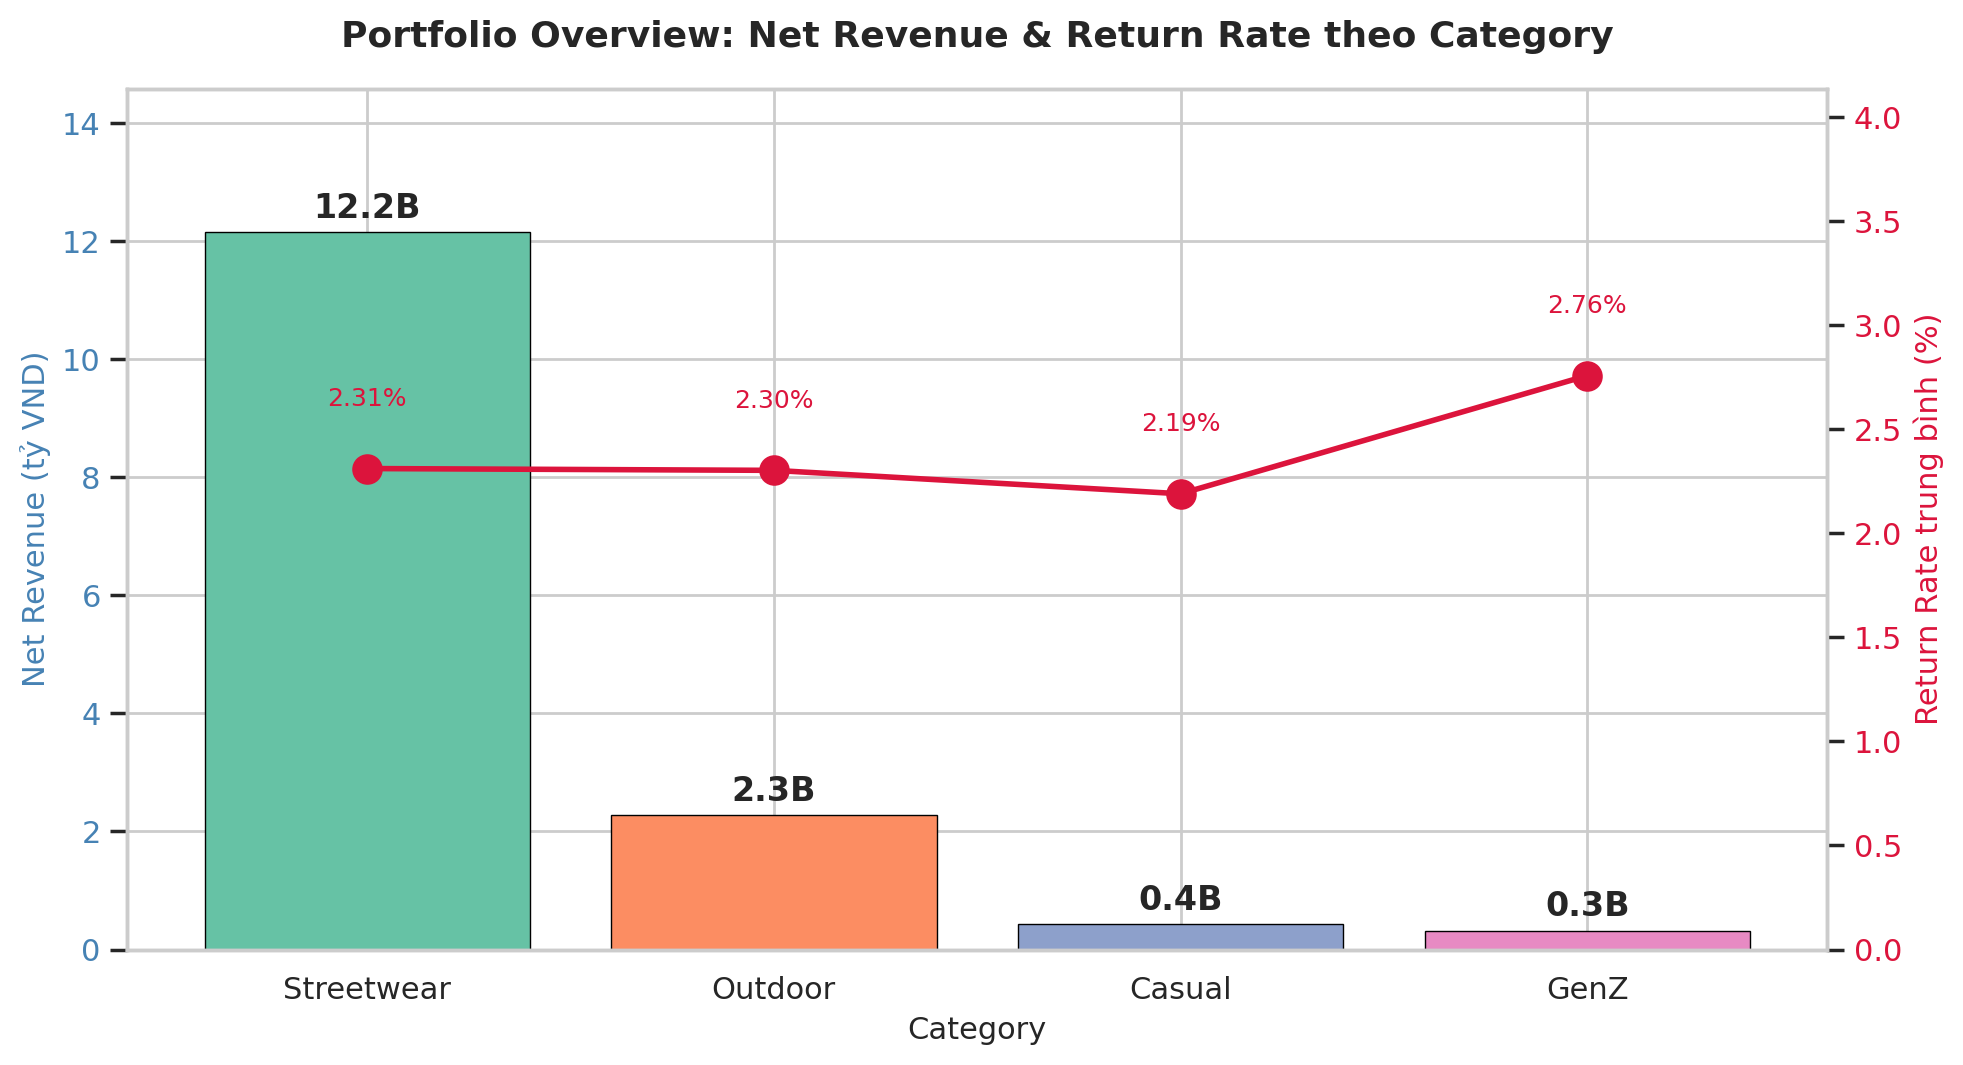
\includegraphics[width=0.72\linewidth]{A_1_1_category_overview.png}
    \caption{Doanh thu thuần và return rate theo Category. Streetwear 75\% portfolio (12.15 tỷ VND), gấp 5.3$\times$ Outdoor; return rate đồng đều 2.2--2.8\% across 4 category $\to$ vấn đề hệ thống.}
    \label{fig:portfolio}
\end{figure}

\textbf{Concentration risk lớn}: Streetwear 75\% revenue (12.15 tỷ); Outdoor 2.27 tỷ với 743 SKUs nhưng under-leveraged. Return rate đồng đều 2.2--2.8\% across 4 category $\to$ \textbf{vấn đề hệ thống, không category-specific}. GenZ (148 SKUs) outlier âm: return cao nhất 2.8\%, margin thấp nhất 24.1\% $\to$ product-market mismatch. \textbf{Customer base}: 87,839 khách, top segment 25--34 tuổi chiếm 28.4\% revenue (Female 14.4\%, Male 14.0\%); Female nhỉnh hơn Male ở mọi nhóm tuổi --- target cho size table fix (§1.2). 18--24 (sinh viên, 6.6\%) là tier tiềm năng nhưng chưa convert hiệu quả.

\subsection{Diagnostic: Wrong Size, COD, \& Mega Sales Failure}

\begin{figure}[H]
    \centering
    \begin{subfigure}[b]{0.54\linewidth}
        \centering
        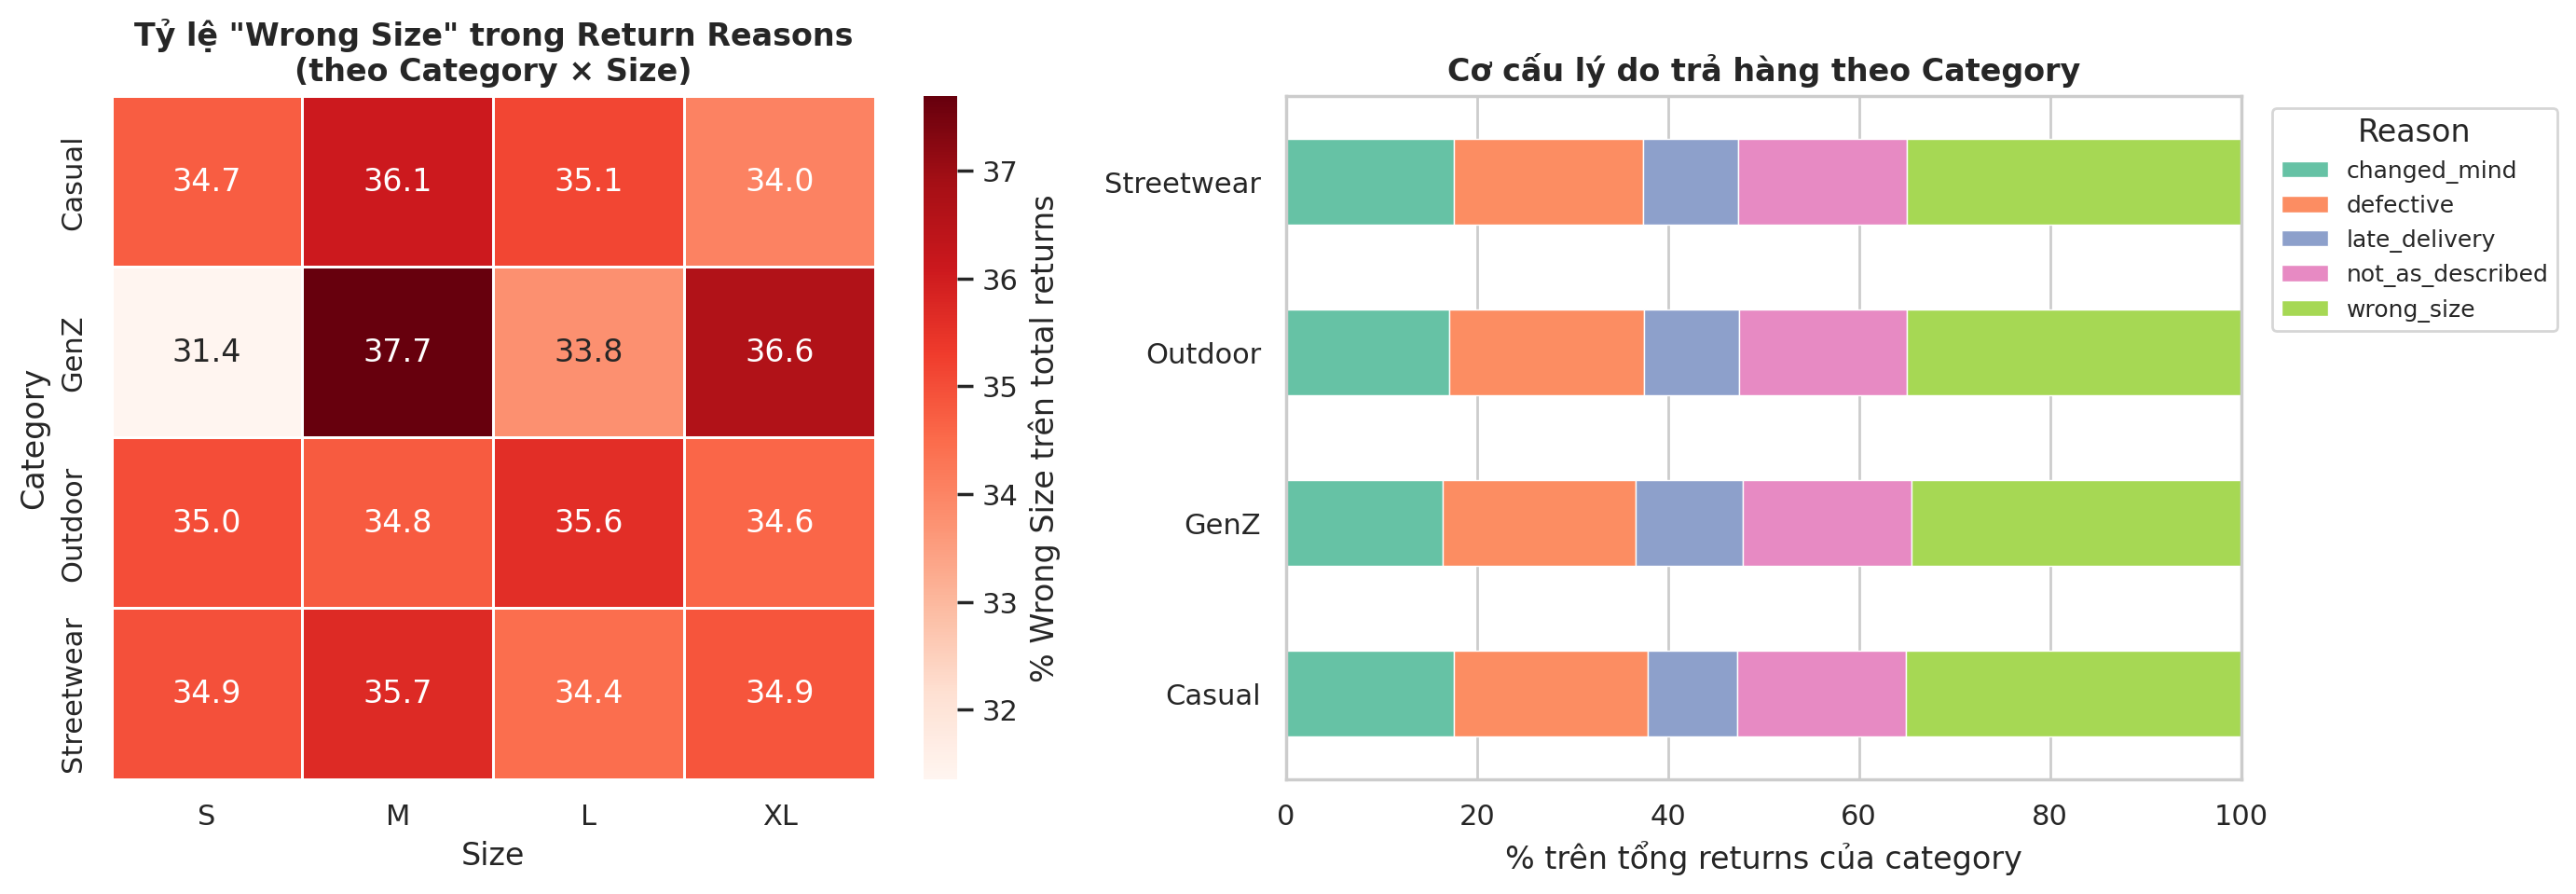
\includegraphics[width=\linewidth]{A_2_1_return_reason_diagnostic.png}
        \caption{Return reasons by Category $\times$ Size: wrong\_size 35\% root cause, đồng nhất 4 category.}
    \end{subfigure}\hfill
    \begin{subfigure}[b]{0.42\linewidth}
        \centering
        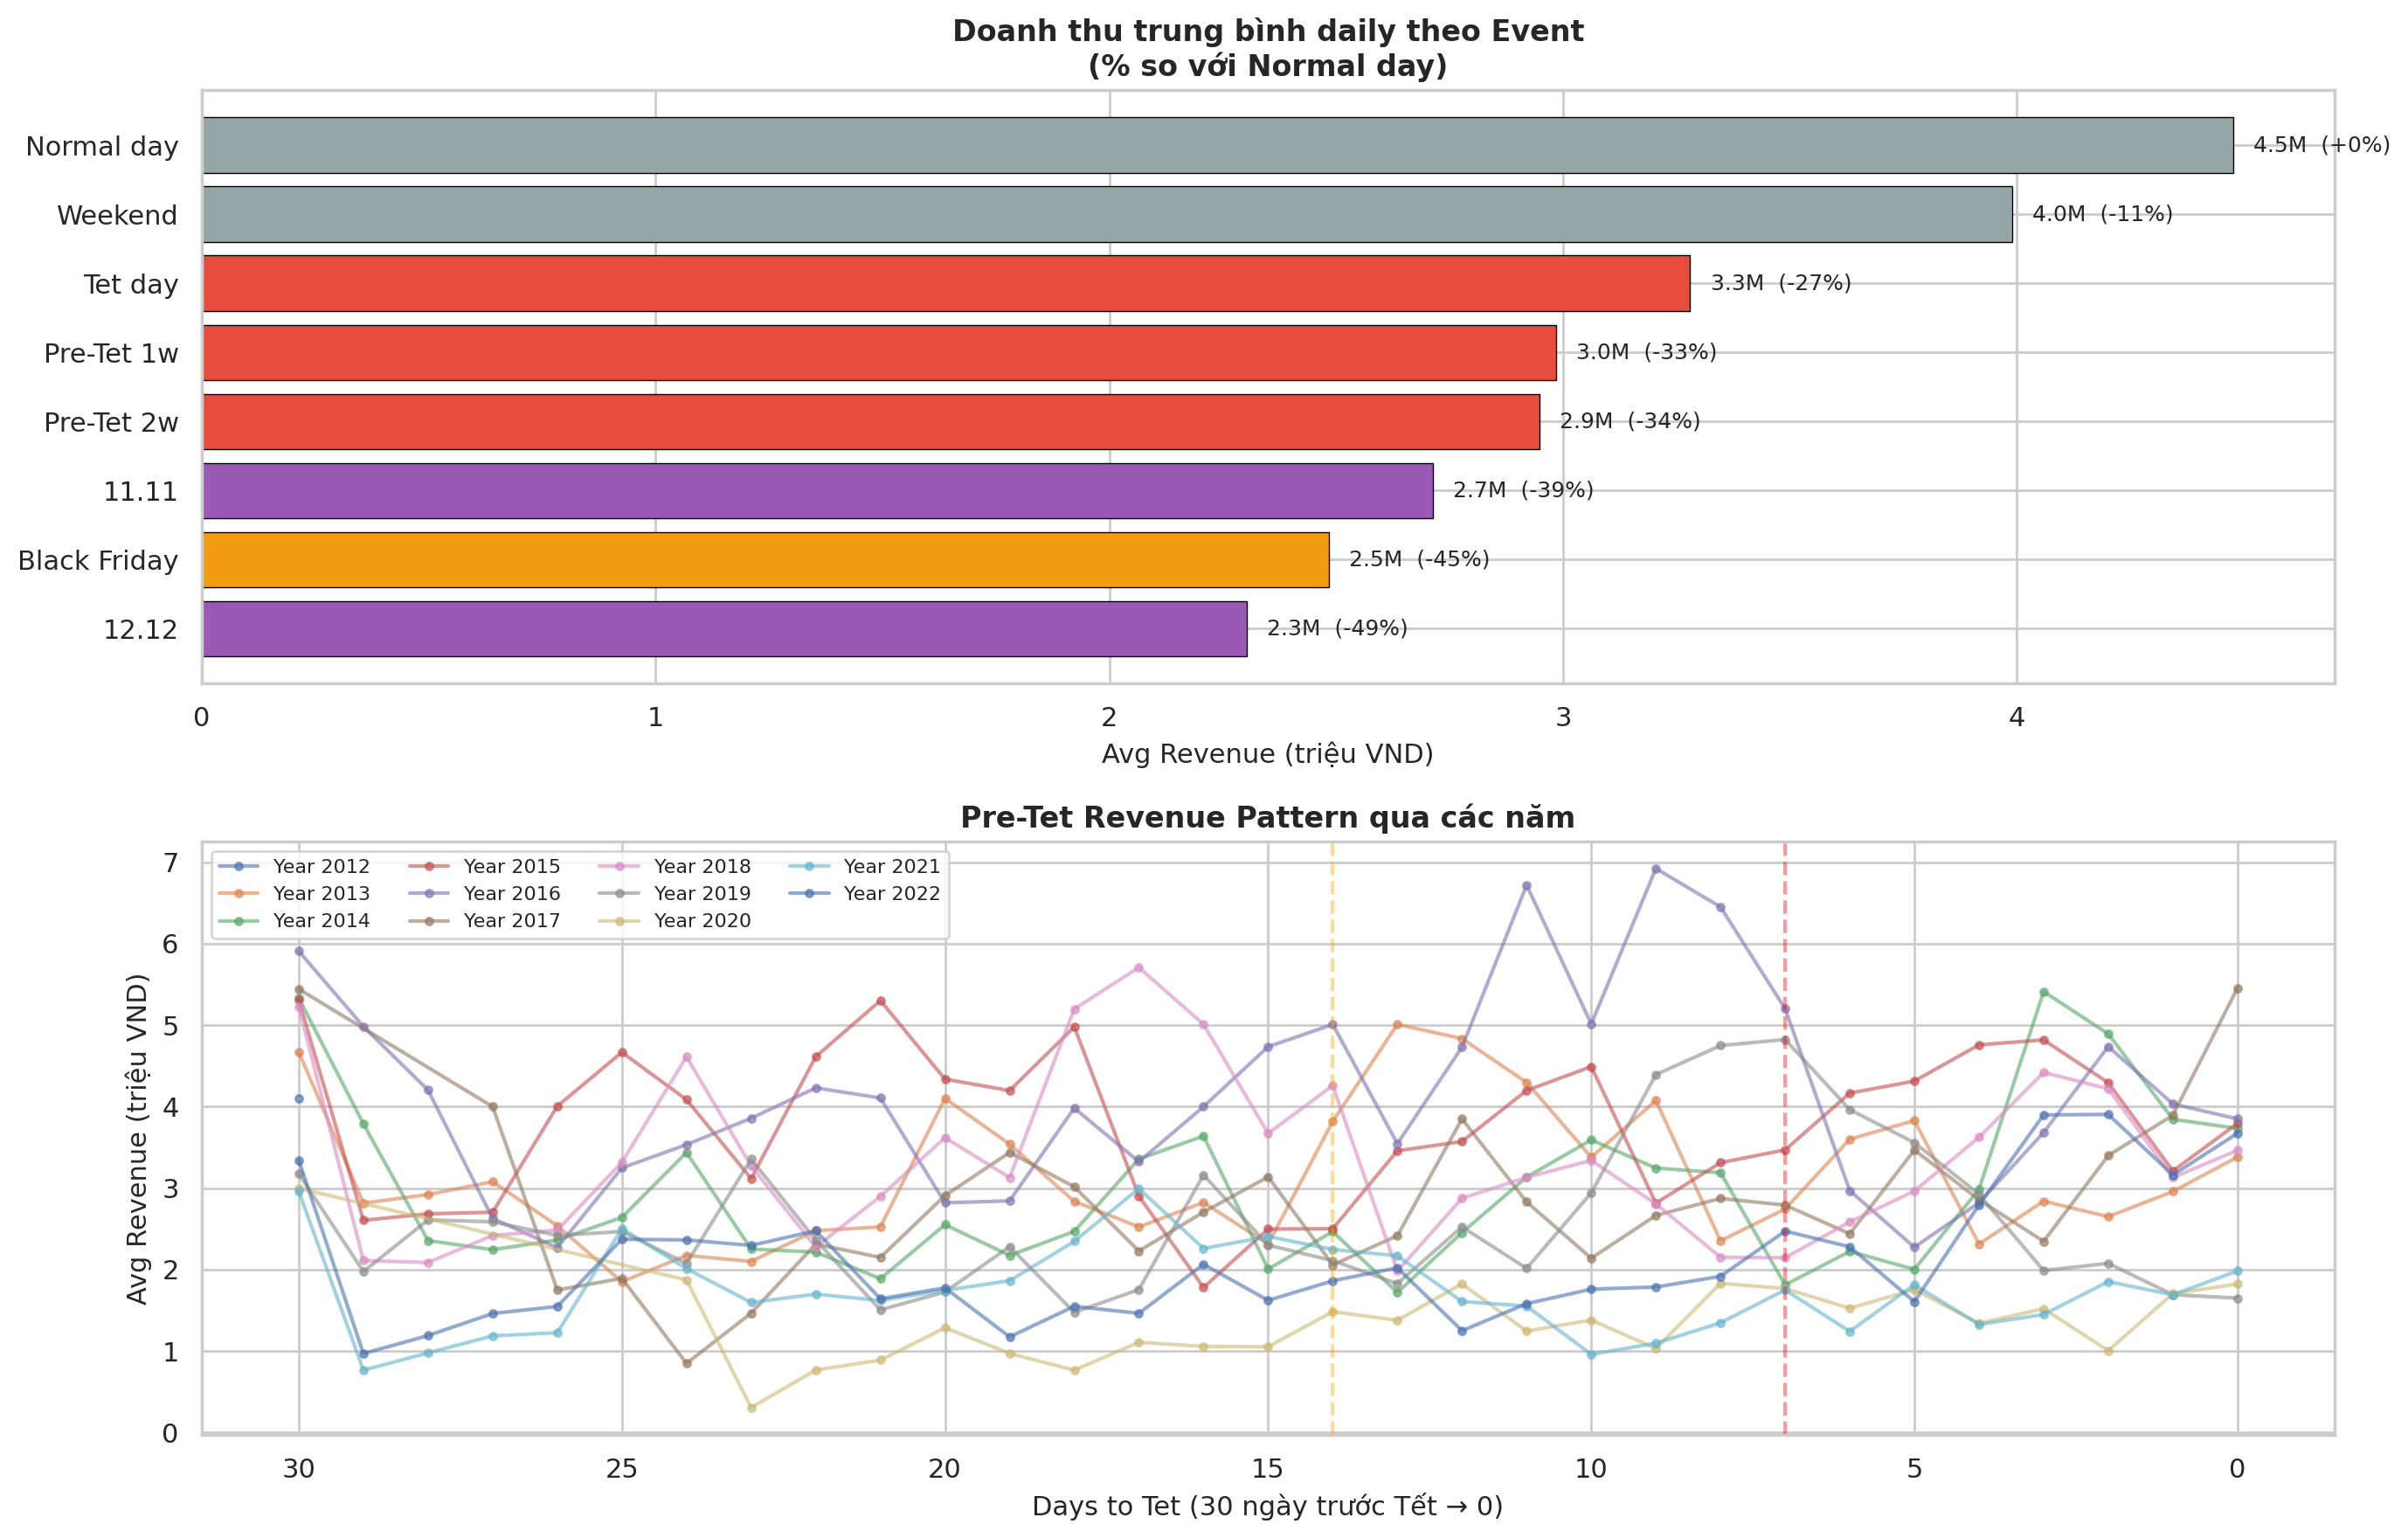
\includegraphics[width=\linewidth]{C_1_2_seasonal_revenue.png}
        \caption{Doanh thu daily theo events: tất cả mega sales VN đều giảm 27--49\% so với normal day 4.48M.}
    \end{subfigure}
    \caption{Diagnostic findings: (a) wrong\_size là root cause hệ thống của returns; (b) mega sales counter-intuitive --- doanh thu \textbf{giảm} 27--49\% trên mọi event.}
    \label{fig:diagnostic}
\end{figure}

\textbf{Wrong\_size = root cause hệ thống}: 35\% returns do size sai, đồng nhất across mọi category $\to$ \textbf{bảng quy đổi size + lack of UX guidance}, không phải chất lượng SP. Defective 20\% + Not\_as\_described 18\% + wrong\_size $=>70\%$ root cause. Casual S/M hotspot (157, 145 returns).
\textbf{COD = bom hủy đơn}: cancel rate 16\% gấp 2$\times$ online (4 phương thức online identical 7.89--8.06\%) $\to$ gap 8pp là vấn đề \textbf{commitment, không UX}. Cost ngầm: 15,468 đơn $\times$ 50--100K = \textbf{750 triệu -- 1.5 tỷ VND/năm}.
\textbf{Mega sales phản tác dụng}: 12.12 ($-49\%$), Black Friday ($-45\%$), 11.11 ($-39\%$), Pre-Tết 2 tuần ($-34\%$), Tết ($-27\%$). Hypotheses: (1) \textbf{Pre-shopping} --- khách biết lịch, mua đón đầu/cắt chờ; (2) \textbf{Discount cannibalization} --- discount sâu kéo gross revenue xuống, đơn không tăng đủ; (3) \textbf{Operational saturation} --- sàn quá tải $\to$ bỏ giỏ. Cross-ref correlation matrix: \texttt{Total\_Discount\_Amount} có $r=0.76$ ($p<0.001$) với \texttt{Returns\_Changed\_Mind} $\to$ discount sâu kích hoạt impulse + đổi ý.

\subsection{Predictive: RFM Segmentation \& Refund Cash-Flow Forecast}

\begin{figure}[H]
    \centering
    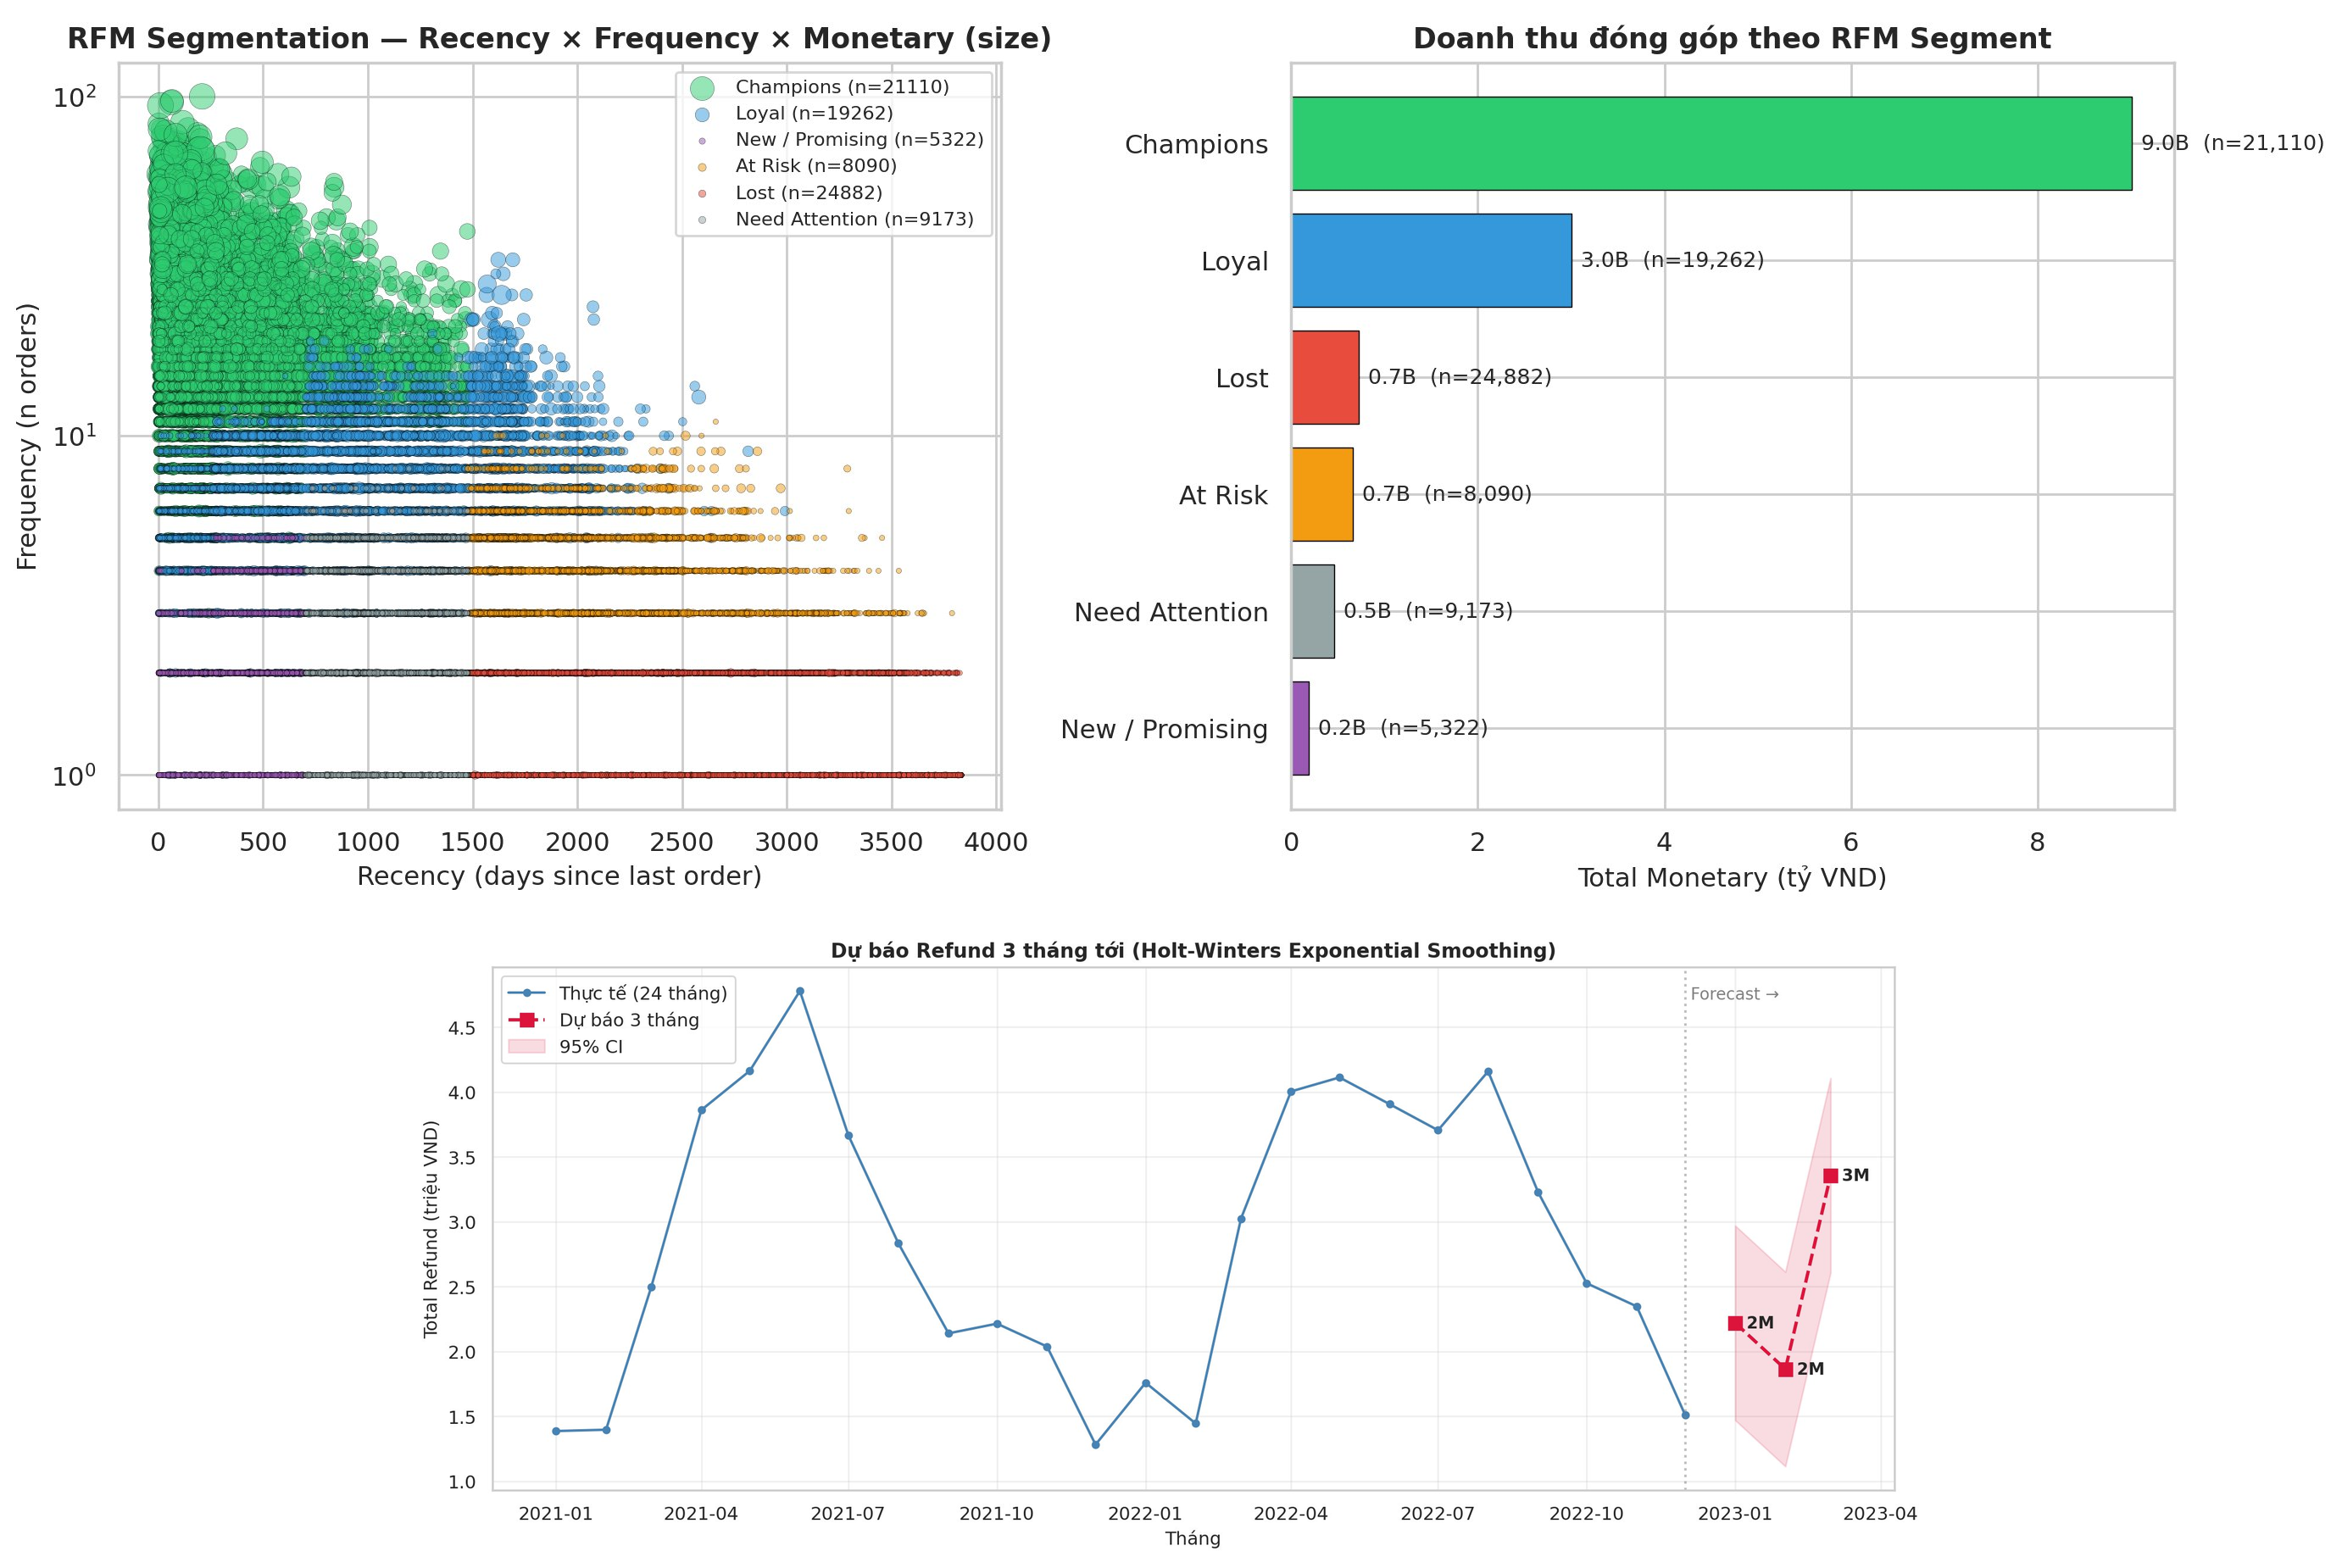
\includegraphics[width=0.78\linewidth]{predictive_rfm_refund.png}
    \caption{Predictive analytics: (top) RFM 6 segments --- Champions 21K (9.0 tỷ), Loyal 19K (3.0 tỷ) là 2 nhóm cốt lõi; At Risk 8K (recency 2,028 ngày) cần win-back. (bottom) Holt-Winters forecast refund 3 tháng tới Q1 2023 với CI 95\%, signal seasonality + trend phục hồi sau dip Q4 2022.}
    \label{fig:predictive}
\end{figure}

\textbf{RFM Segmentation} (Cell B.3.1): \textbf{Champions} 21,110 khách (24\%) đóng góp \textbf{9.0 tỷ} revenue, monetary trung bình 427K --- backbone retention. \textbf{Loyal} 19,262 khách (3.0 tỷ) feeder upgrade Champions. \textbf{At Risk} 8,090 khách (recency 2,028 ngày, monetary 661M) win-back high ROI. \textbf{Lost} 24,882 (recency $>$2,500 ngày) đã churn. New/Promising 5,322 cần convert trước window 90 ngày. \textbf{Risk Tier Classification} (Cell A.3.1): Low 1,355 SKUs (median return 3\%), Medium 213 (6\%), \textbf{High Risk chỉ 30 SKUs} nhưng median return \textbf{24\%} --- ưu tiên QC audit ngay trước Tết.
\textbf{Refund Forecast} (Holt-Winters Exponential Smoothing 24-tháng): predict 3 tháng Q1 2023 với CI 95\%. Pattern phát hiện: refund seasonal (peak Q2 2021 và Q2--Q3 2022 đều $\sim$4M triệu VND), trough cuối năm. Forecast cho thấy Q1 2023 refund sẽ \textbf{phục hồi từ dip Q4 2022} ($\sim$1.5M) lên $\sim$2--3M, tiếp nối seasonal cycle. Combo với Risk Tier: \textbf{30 High Risk SKUs là driver chính} của refund spike --- cắt return của nhóm này trước Tết để giảm refund peak Q1.

\subsection{Prescriptive: Action Portfolio + Top 5 Concrete Actions}

\begin{figure}[H]
    \centering
    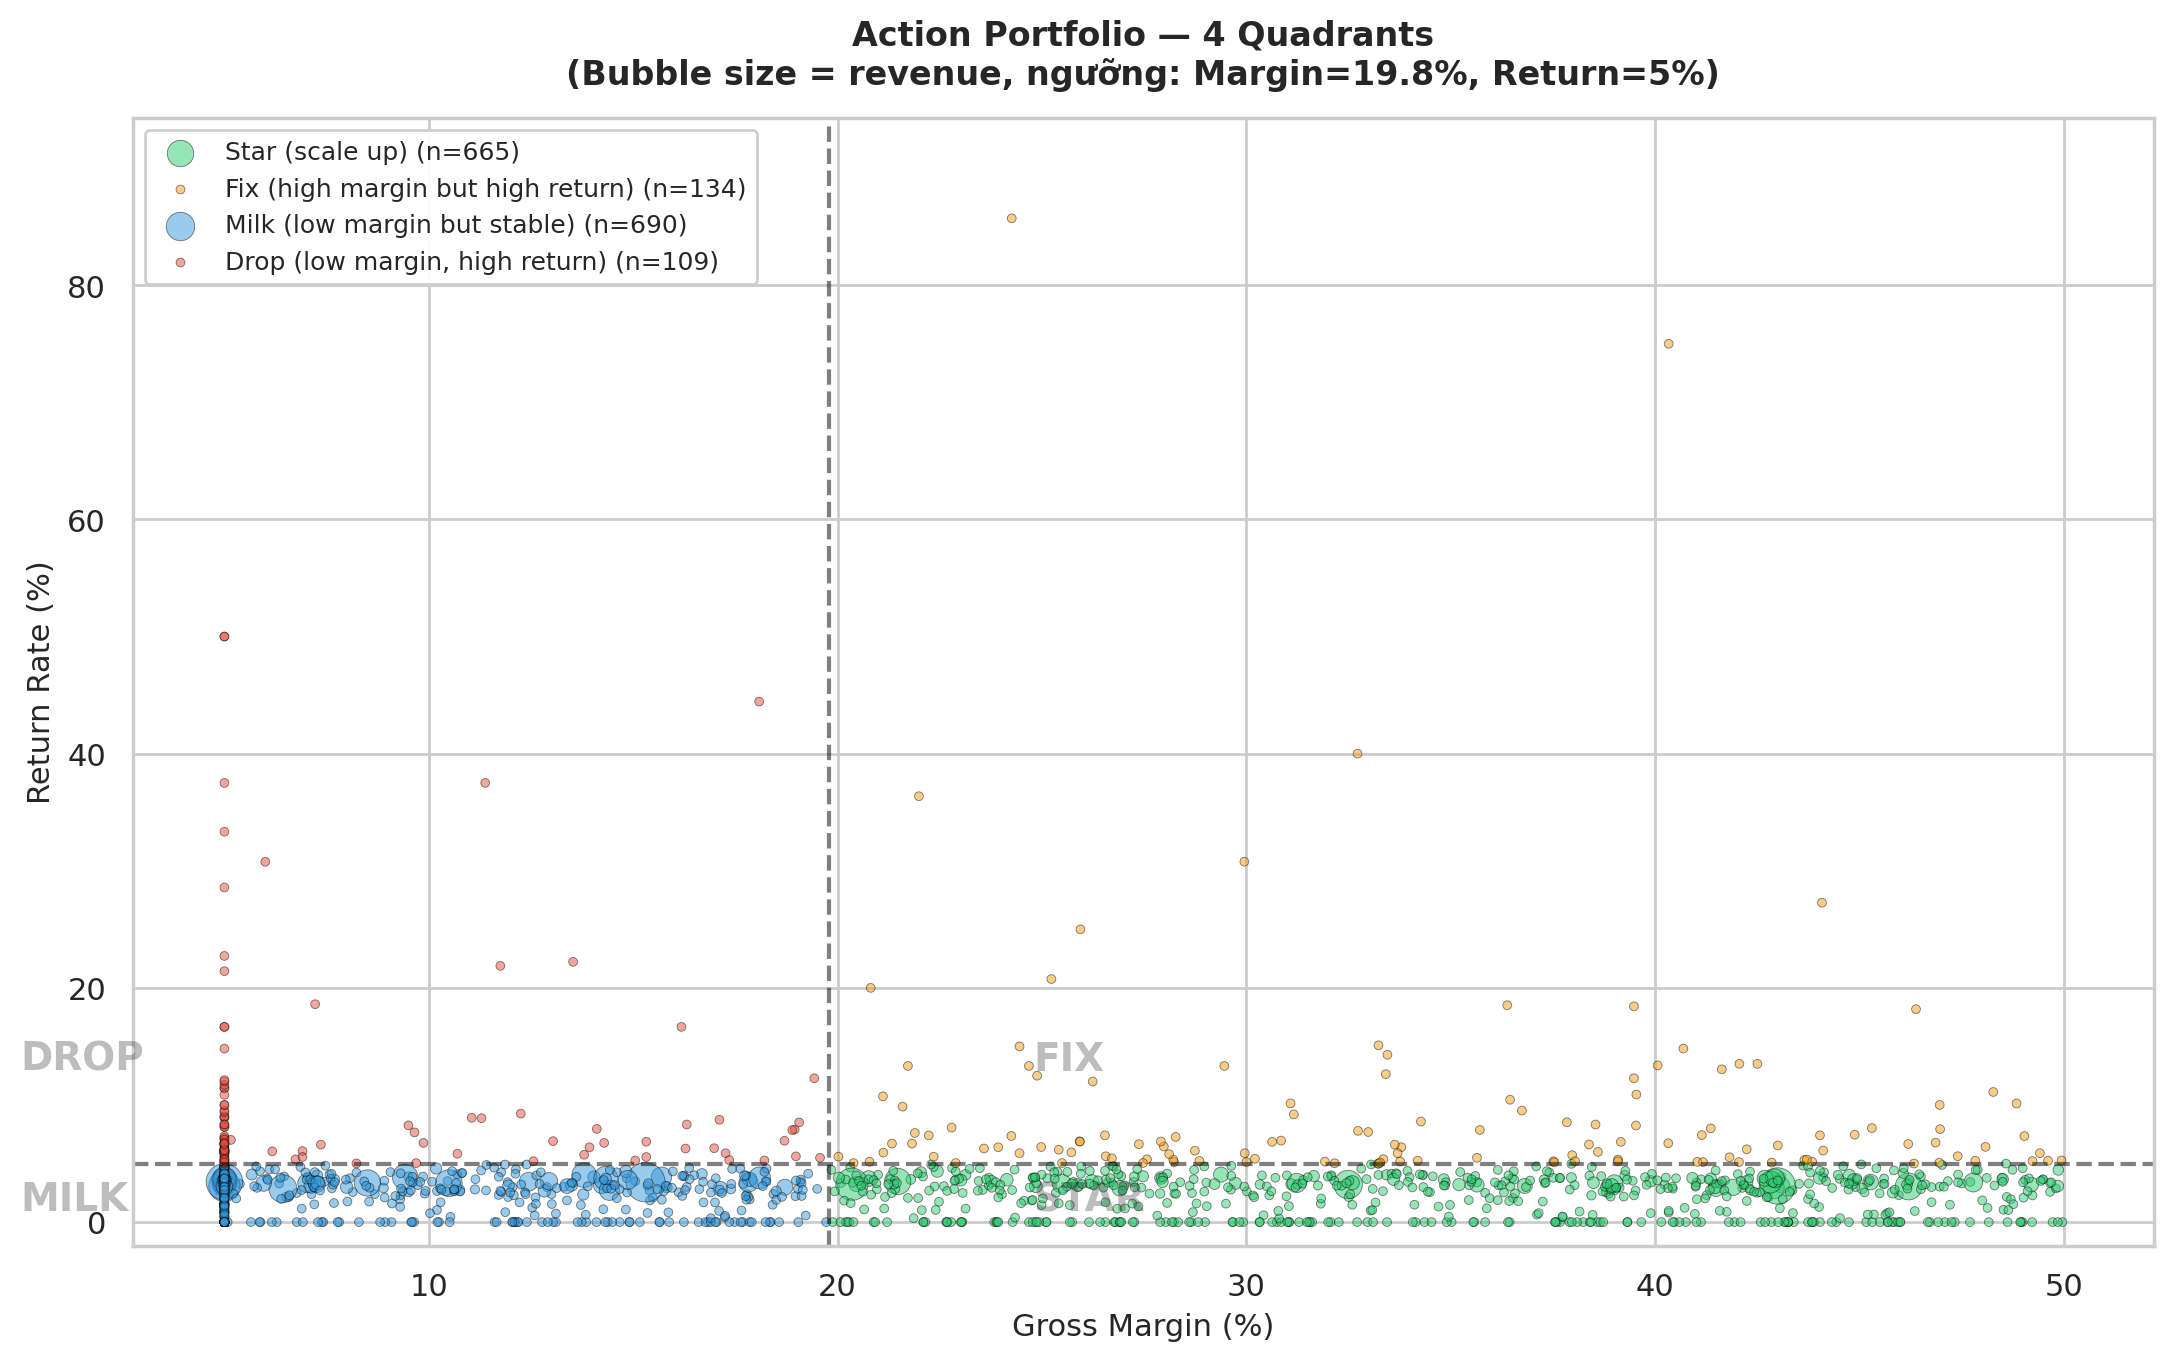
\includegraphics[width=0.50\linewidth]{A_4_1_action_quadrant.png}
    \caption{Action Portfolio Quadrant 1,598 SKUs (Margin 19.8\%, Return 5\%): Star 665, Milk 690, Fix 134, Drop 109.}
    \label{fig:prescriptive}
\end{figure}

\textbf{SKU Quadrant}: Star 665 (41.6\%) backbone Streetwear --- protect+scale; Milk 690 (43.2\%) bundle với Star tăng AOV; Fix 134 (8.4\%) Streetwear premium bị wrong\_size returns $\to$ margin tiềm năng nếu fix size; Drop 109 (6.8\%) đốt tiền kép $\sim$700 triệu refund/năm. \textbf{Channel Quality} (\% Champions+\% Loyal): organic\_search 86.4 (3.93 tỷ rev), paid\_search 73.7, social\_media 72.0, email 48.6, direct 38.5, referral 35.4 $\to$ \textbf{gap 51pp}. Search-based thắng vì intent-driven traffic, direct/referral incidental.
\textbf{Top 5 Actions 2023} (impact: $+1.7$--$1.8$ tỷ revenue, $-500$ triệu cost): \textbf{(1) Portfolio cleanup} --- Drop 109 SKUs liquidation 30 ngày, Fix 134 SKUs 60-day rescue (giải phóng 700 triệu refund); \textbf{(2) AI size recommender} ưu tiên Casual S/M (30 triệu logistics + uy tín); \textbf{(3) COD verification} SMS/IVR $>500$K VND + discount prepaid 2--3\% (250--500 triệu/năm); \textbf{(4) Marketing reallocation} $+30$--$40\%$ organic/paid\_search, $-30\%$ direct/referral; tăng \%Champions $24\%\to28\%$ ($+3,500 \times 427$K $= +1.5$ tỷ); \textbf{(5) Promo calendar 2023} --- stop 12.12, cắt 80\% Black Friday, Tết chỉ 3--4 ngày, A/B test 11.11 với 50\% intensity (tiết kiệm 60--70\% promo budget). \textbf{Risk Tier guard}: 30 High Risk SKUs (§1.3) cần QC audit 100\% trước Tết để cắt refund peak Q1 (theo seasonal forecast).


\section{Sales Forecasting (Phần 3)}

\subsection{Pipeline kiến trúc Hybrid Multi-Layer}

Dự báo Revenue và COGS theo ngày cho 2023-01-01 đến 2024-07-01 (548 ngày), train trên 2012-07-04 đến 2022-12-31 (3,287 ngày). Đánh giá MAE, RMSE, $R^2$. Đề xuất kiến trúc 4 lớp:

\begin{enumerate}[leftmargin=*,itemsep=1pt,topsep=2pt]
    \item \textbf{Baseline}: $\hat{y}_t = \mu_{base} \cdot g^{\Delta y} \cdot s_{m,d}$ với $g$ geometric mean growth, $s_{m,d}$ seasonal index theo (month, day).
    \item \textbf{Cross-table features}: 23 daily share ratios từ 4 dim tables (region/payment/device/source/status); test không có dim data $\to$ impute (month, dow) lookup từ train post-2020.
    \item \textbf{Macro events}: 5 cờ regime (growth\_era, 2019\_slowdown, covid\_lockdown, post\_lockdown\_recovery, inflation\_2022) --- chỉ áp COGS theo ablation.
    \item \textbf{Alpha-shrinkage}: $\hat{y}_{final} = \hat{y}_{baseline} + \alpha \cdot \hat{r}_{ML}$, $\alpha < 1$ chống overfit (Stein-like). ML residual: XGBoost cho Revenue, CatBoost cho COGS theo per-target CV.
\end{enumerate}

\subsection{Cross-Validation đúng chiều thời gian \& Ablation}

CV time-series 2 fold rolling-origin (train $\leq 2020$, val=2021; train $\leq 2021$, val=2022; bỏ COVID 2020 outlier). \textbf{No leakage}: baseline được fit lại từ đầu cho mỗi fold với upper\_year $= y-1$, dim features impute từ post-2020 train data. Tối ưu $\alpha$ qua \textit{combined score} $= \frac{\Delta MAE}{MAE_b} + \frac{\Delta RMSE}{RMSE_b} + (R^2 - R^2_b)$. Kết quả: $\alpha_{rev}=0.350$, $\alpha_{cogs}=0.275$.

\begin{table}[H]
\centering
\small
\caption{Ablation study CV (2 folds 2021+2022).}
\label{tab:ablation}
\begin{tabular}{lcccc}
\toprule
\textbf{Approach} & \textbf{Rev MAE} & \textbf{Rev R\textsuperscript{2}} & \textbf{COGS MAE} & \textbf{COGS R\textsuperscript{2}} \\
\midrule
Original notebook (rank 1902)        & 583K & 0.7587 & 544K & 0.7194 \\
Baseline only                        & 597K & 0.7663 & 489K & 0.7821 \\
Baseline + Alpha-shrinkage           & 569K & 0.7773 & 476K & 0.7871 \\
+ Cross-table features (Plan A)      & 564K & 0.7823 & 476K & 0.7878 \\
\textbf{+ Macro events (COGS only)}  & \textbf{564K} & \textbf{0.7823} & \textbf{471K} & \textbf{0.7916} \\
\bottomrule
\end{tabular}
\end{table}

\subsection{SHAP, Compliance \& Reproducibility}

\begin{figure}[H]
    \centering
    \begin{subfigure}[b]{0.36\linewidth}
        \centering
        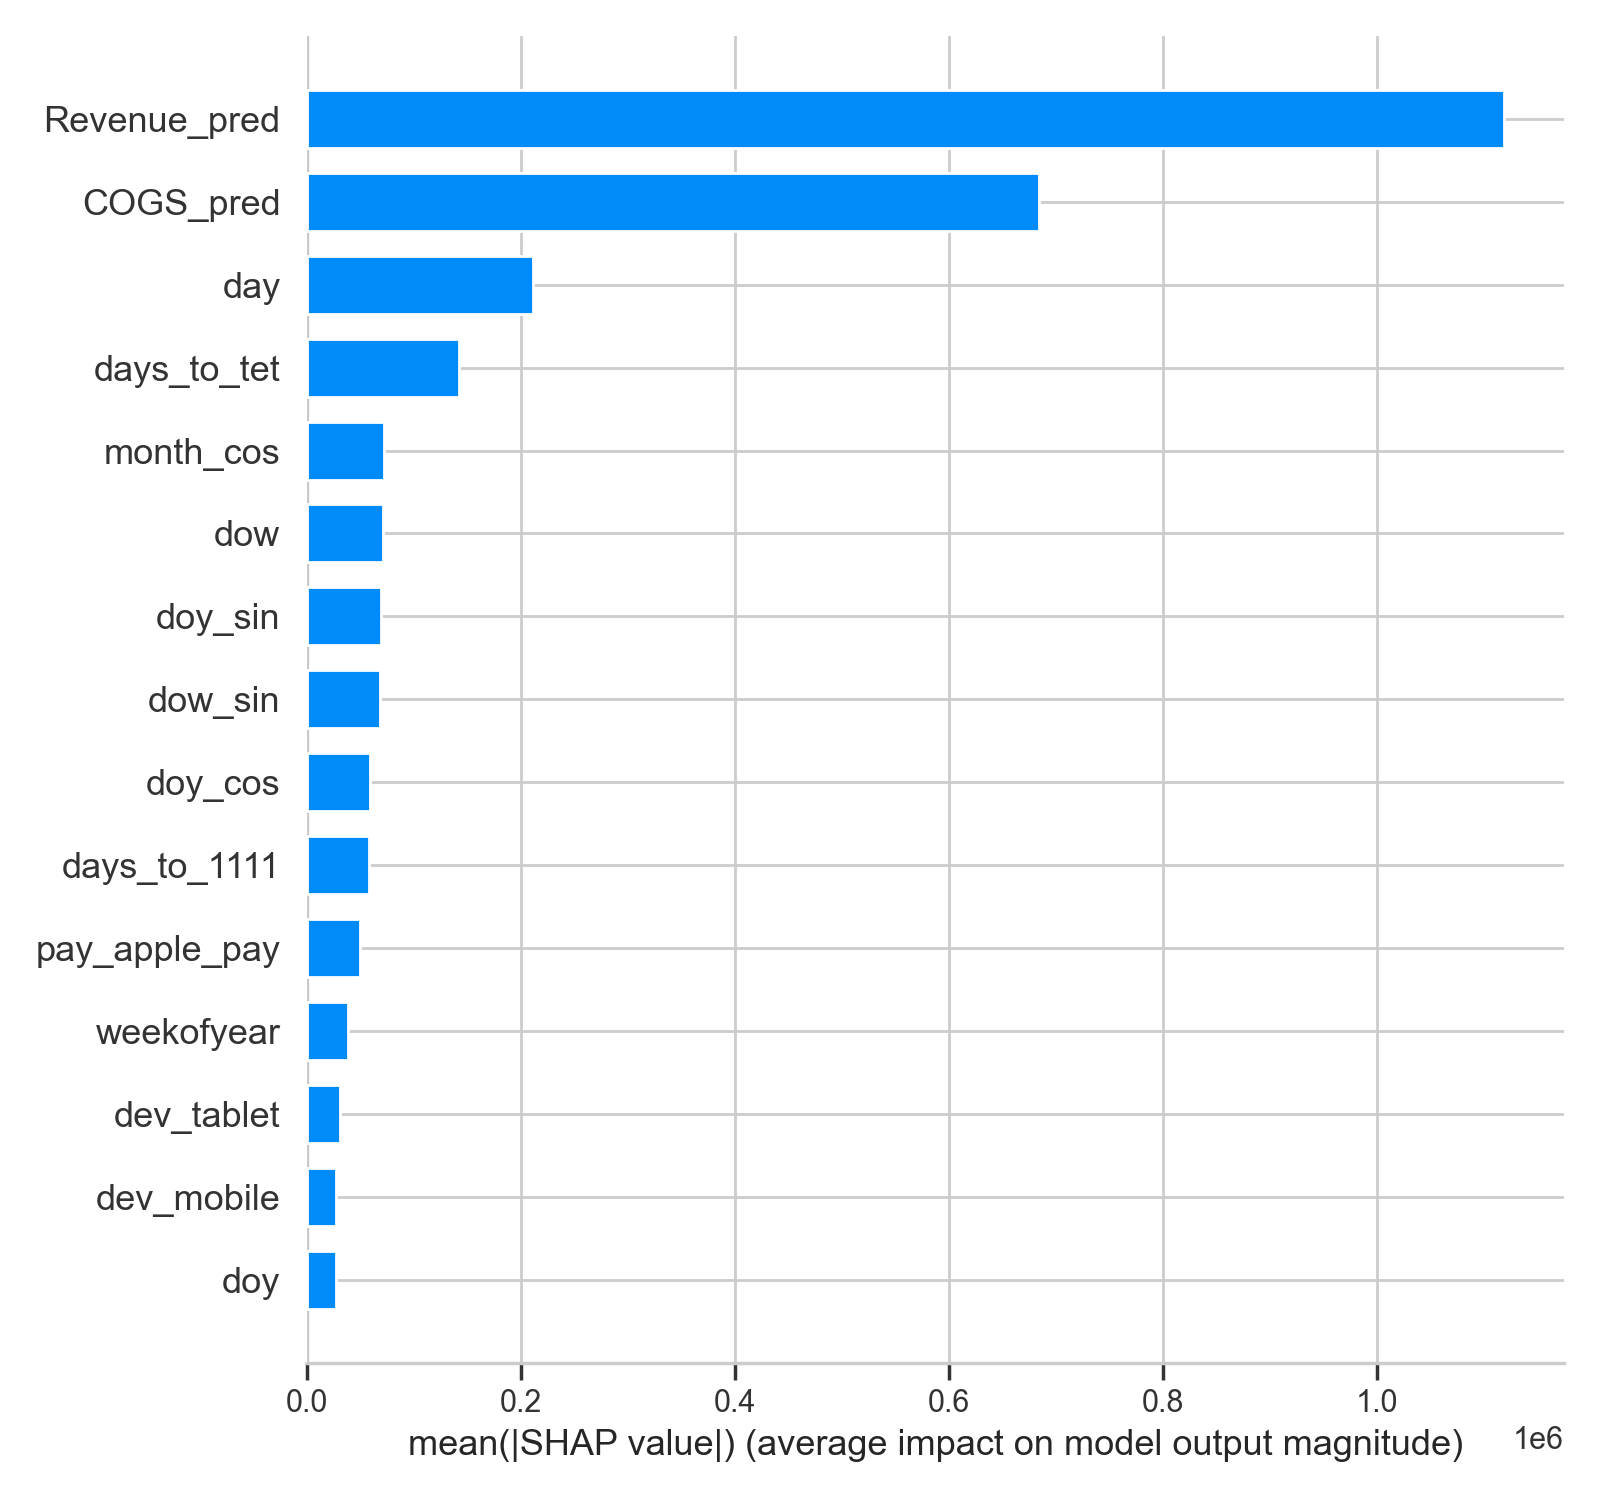
\includegraphics[width=\linewidth]{shap_revenue.png}
        \caption{SHAP Revenue residual (XGBoost, fold val=2022).}
        \label{fig:shap}
    \end{subfigure}\hfill
    \begin{subfigure}[b]{0.62\linewidth}
        \centering
        
\includegraphics[width=\linewidth]{forecast_overview.png}
        \caption{Forecast Revenue/COGS 2023-01 đến 2024-07 (đỏ) kế thừa seasonal từ historical (xám).}
        \label{fig:forecast}
    \end{subfigure}
    \caption{(a) Feature importance cho Revenue residual; (b) Forecast 548 ngày, predictions ổn định.}
    \label{fig:shap-forecast}
\end{figure}

\textbf{Top-5 SHAP Revenue} (XGB): \texttt{Revenue\_pred} (1.12M), \texttt{COGS\_pred} (684K), \texttt{day} (211K), \texttt{days\_to\_tet} (142K), \texttt{month\_cos} (72K). \textbf{Top-5 SHAP COGS} (CatBoost): \texttt{COGS\_pred} (1.01M), \texttt{Revenue\_pred} (573K), \texttt{day} (157K), \texttt{is\_growth\_era} (153K), \texttt{is\_2019\_slowdown} (122K). Baseline dominate $\to$ ML học residual; \texttt{day}+\texttt{days\_to\_tet} là signal phi-tuyến (payday+Tết); macro events top-5 COGS confirms ablation $\to$ COGS nhạy cảm regime kinh tế. \textbf{Compliance 3 ràng buộc}: (i) \texttt{FEATS\_REV}/\texttt{FEATS\_COG} không chứa Revenue/COGS (mart4 test=NaN). (ii) Chỉ load file provided; macro flags là date-based encoding. (iii) seed=42, deterministic folds, notebook \texttt{04\_MLE\_KILLER\_FINAL.ipynb}. \textbf{Code \& Reproducibility}: GitHub repo \url{https://github.com/LineLuLan/The-Richers} (notebooks, mart-builders, submission).

\end{document}